              
% --------------------------------------------------------------
% This is all preamble stuff that you don't have to worry about.
% Head down to where it says "Start here"
% --------------------------------------------------------------
 
\documentclass[11pt]{article}
\usepackage[utf8]{inputenc} 
\usepackage[margin=1in]{geometry}
\usepackage{graphicx}
\usepackage{float}
\usepackage{hyperref} 
\usepackage{amsmath,amsthm,amssymb}
\usepackage[table]{xcolor}
 
\newcommand{\N}{\mathbb{N}}
\newcommand{\Z}{\mathbb{Z}}
 
\newenvironment{theorem}[2][Theorem]{\begin{trivlist}
\item[\hskip \labelsep {\bfseries #1}\hskip \labelsep {\bfseries #2.}]}{\end{trivlist}}
\newenvironment{lemma}[2][Lemma]{\begin{trivlist}
\item[\hskip \labelsep {\bfseries #1}\hskip \labelsep {\bfseries #2.}]}{\end{trivlist}}
\newenvironment{exercise}[2][Exercise]{\begin{trivlist}
\item[\hskip \labelsep {\bfseries #1}\hskip \labelsep {\bfseries #2.}]}{\end{trivlist}}
\newenvironment{reflection}[2][Reflection]{\begin{trivlist}
\item[\hskip \labelsep {\bfseries #1}\hskip \labelsep {\bfseries #2.}]}{\end{trivlist}}
\newenvironment{proposition}[2][Proposition]{\begin{trivlist}
\item[\hskip \labelsep {\bfseries #1}\hskip \labelsep {\bfseries #2.}]}{\end{trivlist}}
\newenvironment{corollary}[2][Corollary]{\begin{trivlist}
\item[\hskip \labelsep {\bfseries #1}\hskip \labelsep {\bfseries #2.}]}{\end{trivlist}}
 
\begin{document}
 
% --------------------------------------------------------------
%                         Start here
% --------------------------------------------------------------
 
\setlength\parindent{0pt}
%\renewcommand{\qedsymbol}{\filledbox}
 
\title{Assignment 2: Evolutionary dynamics in a spatial context}%replace X with the appropriate number
\author{Pierre Gérard (ULB)\\ %replace with your name
INFO-F-409 - Learning dynamics} %if necessary, replace with your course title
 
\maketitle

\section{Part 1}
For this part, the selected game is the Prisoners Dilemna (T=10, R=7, P=0, S=0). Two actions are possible for a player : Cooperate or defect. A player payoff is the sum of the game against its 8 neighbours at first. Each player will basically copy at every turn the action of his neighbour getting the best payoff.

\subsection{Cooperation level}

\subsubsection{Plot}

\begin{figure}[H]
   \centering
   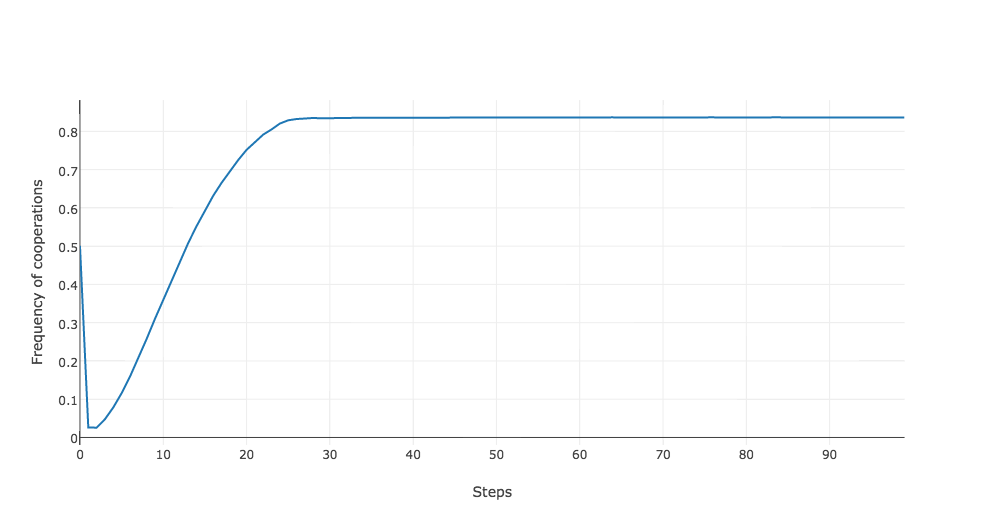
\includegraphics[width=0.8\textwidth]{img/part1/cf-moore-notmyself.png}
\end{figure}

In the plot above, we can see the frequency of cooperation (i.e. the fraction of player cooperating). We can see that starting at $0.5$, it first goes down before going up again and stabilizing at around $0.84$.

\subsubsection{Same in every run ?}

\begin{figure}[H]
\centering
   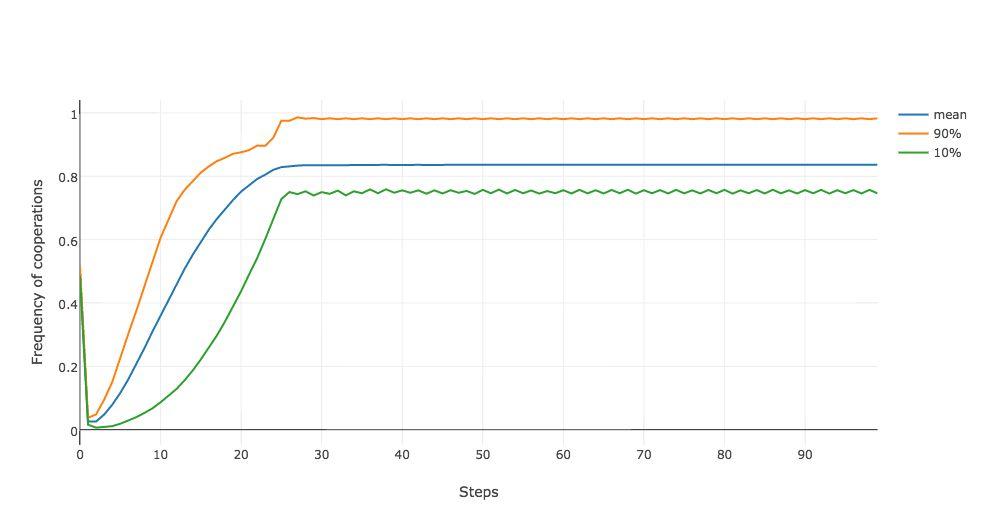
\includegraphics[width=0.8\textwidth]{img/part1/cf-moore-notmyself-90-10.png}
\end{figure}

Answering the question \textit{is it approximately the same} is quite hard because it can be subjective. Above, it is plotted the $0.1$ and $0.9$ quantile. From this plot, one could reasonably say that it is in fact "approximately the same". Note that the $0.1$ and $0.9$ quantile has been chosen because the minimum would be at $0$ and the maximum at $1$.

\subsection{Visualization}

In the visualization below, red is cooperation and blue is defection. We can see some "clusters" getting formatted.

\subsubsection{t=0}

\begin{figure}[H]
\centering
   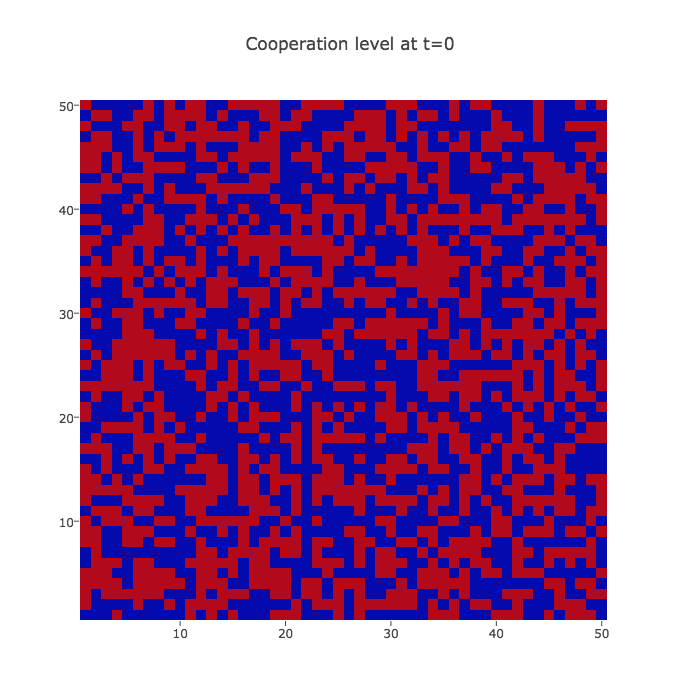
\includegraphics[width=0.6\textwidth]{img/part1/cf-moore-visu-0.png}
\end{figure}

\subsubsection{t=1}

\begin{figure}[H]
\centering
   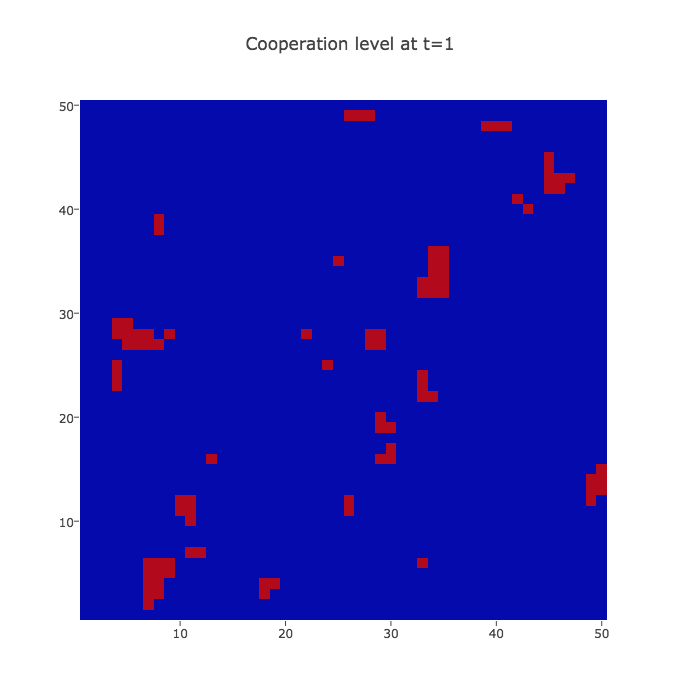
\includegraphics[width=0.6\textwidth]{img/part1/cf-moore-visu-1.png}
\end{figure}

\subsubsection{t=5}

\begin{figure}[H]
\centering
   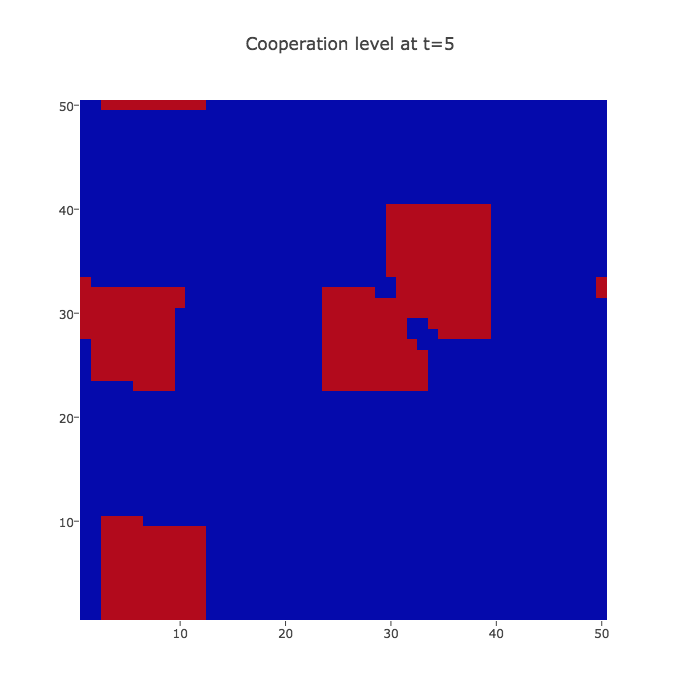
\includegraphics[width=0.6\textwidth]{img/part1/cf-moore-visu-5.png}
\end{figure}

\subsubsection{t=10}

\begin{figure}[H]
\centering
   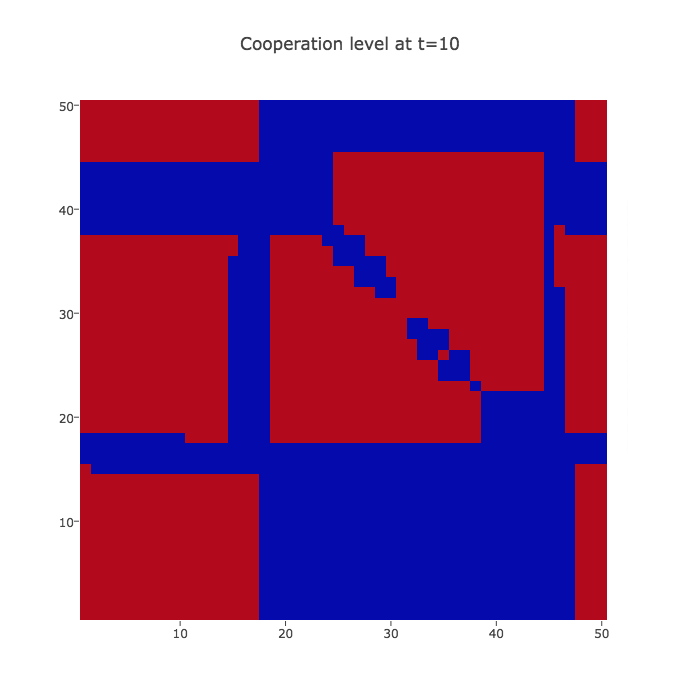
\includegraphics[width=0.6\textwidth]{img/part1/cf-moore-visu-10.png}
\end{figure}

\subsubsection{t=20}

\begin{figure}[H]
\centering
   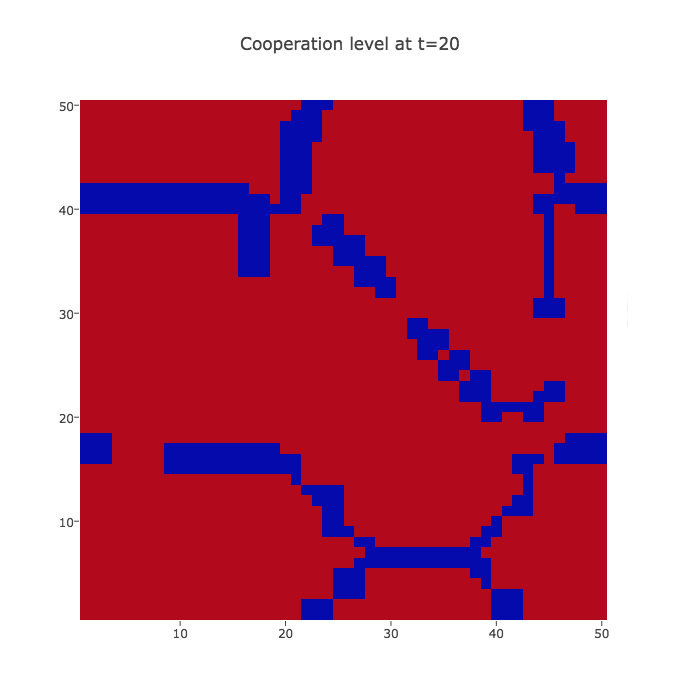
\includegraphics[width=0.6\textwidth]{img/part1/cf-moore-visu-20.png}
\end{figure}

\subsubsection{t=50}

\begin{figure}[H]
\centering
   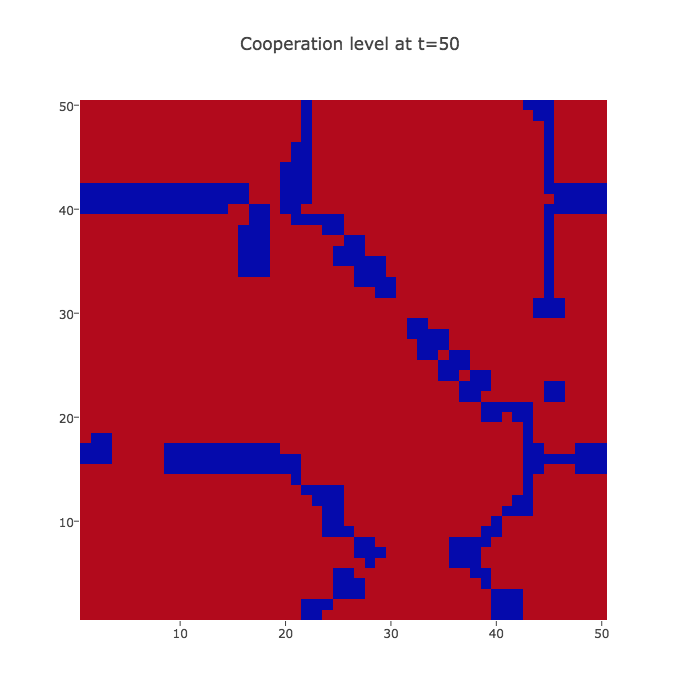
\includegraphics[width=0.7\textwidth]{img/part1/cf-moore-visu-50.png}
\end{figure}

\subsection{Lattice size}

\subsubsection{4x4}

\begin{figure}[H]
\centering
   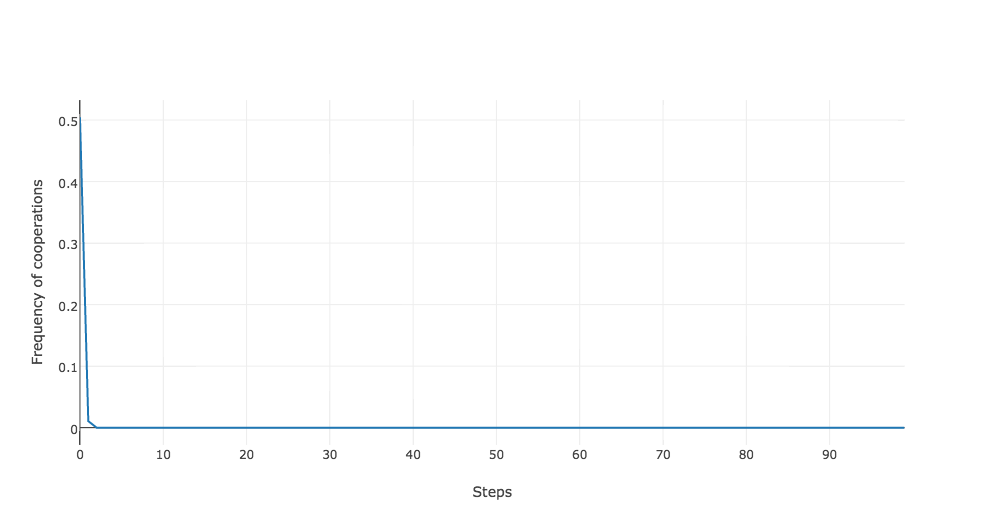
\includegraphics[width=0.6\textwidth]{img/part1/cf-moore-4-4.png}
\end{figure}

\subsubsection{8x8}

\begin{figure}[H]
\centering
   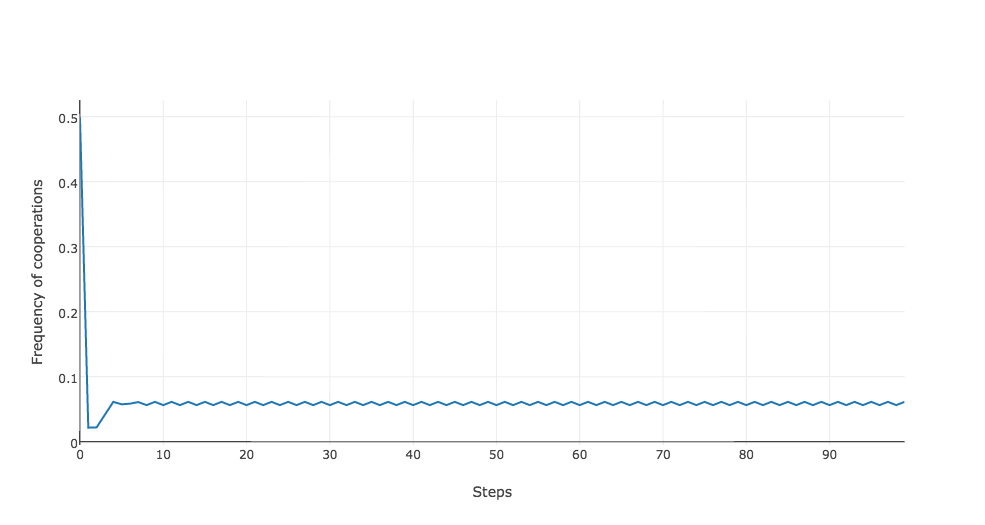
\includegraphics[width=0.6\textwidth]{img/part1/cf-moore-8-8.png}
\end{figure}

\subsubsection{12x12}

\begin{figure}[H]
\centering
   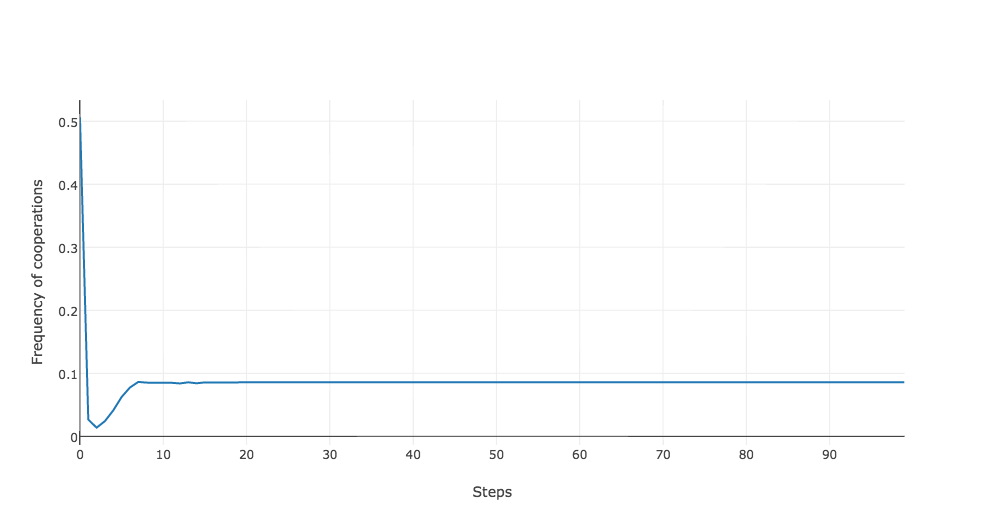
\includegraphics[width=0.6\textwidth]{img/part1/cf-moore-12-12.png}
\end{figure}

\subsubsection{20x20}

\begin{figure}[H]
\centering
   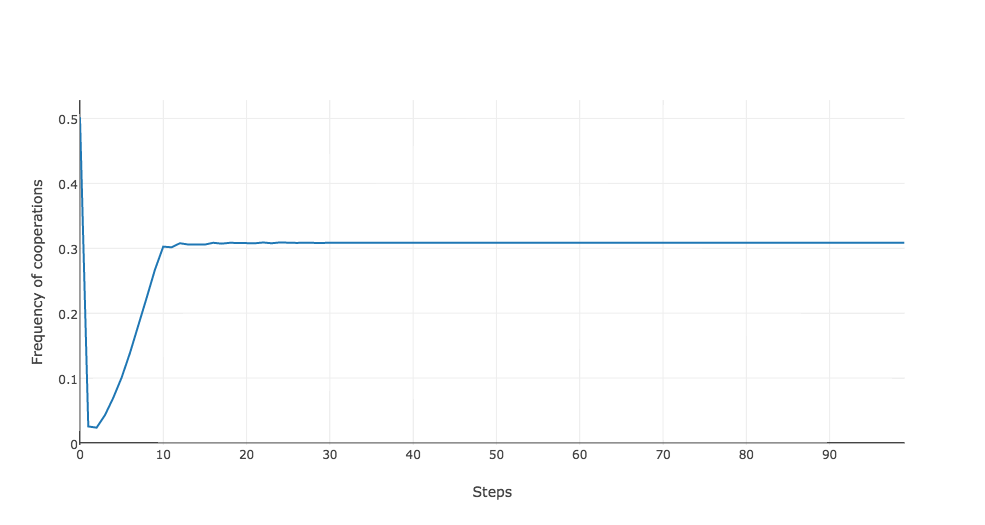
\includegraphics[width=0.6\textwidth]{img/part1/cf-moore-20-20.png}
\end{figure}

\subsubsection{Explanation}

One possible explanation for this outcome is that the smaller is the lattice, the less probable it is to find clusters of cooperation (small zone of cooperation that can get bigger) in the lattice, thus resulting in a smaller cooperation level because cluster reduce exploitation by defectors. Moreover, for example, in a lattice of 4x4, a neighbourhood of 9 equals more than half of the lattice, making it harder to cooperate instead of cheating (more individual). Indeed, the reason for one to cooperate is that is neighbour is cooperating and that the neighbour's neighbour is cooperating and so on.

\subsection{Von Neumann}

\subsubsection{Plot}
\begin{figure}[H]
\centering
   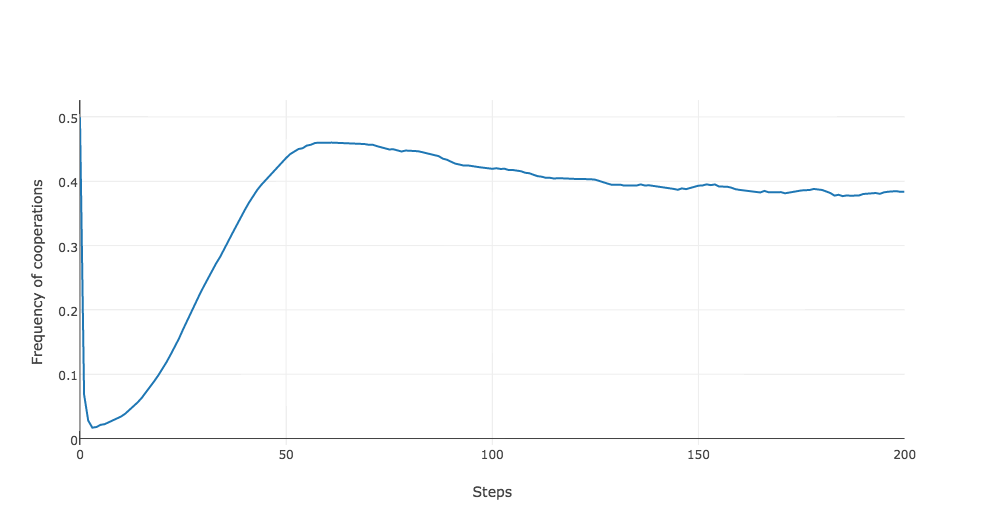
\includegraphics[width=0.8\textwidth]{img/part1/cf-vonn-notmyselfincluded.png}
\end{figure}

\subsubsection{Explanation}
 
A possible explanation for the lower score than with Moore neighbourhood is that the spatial structure are less dense than with moore resulting in an higher incentive to deceive. 
 
\section{Part 2}

\subsection{Probability defined}

$Pij = \frac{1 + [W_j-W_i]/[N*(max\{P,R,T,S\} - min\{P,R,T,S\})]}{2}$ 

This probability makes sense to be defined like that because it indicate the incentive a player has to change is strategy. In other words, the more it can gain by changing his strategy, the more probable he is to change his strategy and will also give him flexibility. 

Indeed, $[W_j-W_i]$ is the payoff difference between the player and his neighbours while $ [N*(max\{P,R,T,S\} - min\{P,R,T,S\})]$ is the maximum possible payoff between player and its neighbours. The interesting part of the fraction is $[W_j-W_i]/[N*(max\{P,R,T,S\} - min\{P,R,T,S\})]$ : it will be equals to 0 if the payoff of the player and his neighbour are equal, negative if the payoff of the player is greater than its neighbour and positive if the payoff of the player is less than its neighbour. The $N$ is there because $[W_j-W_i]$ is proportional to the number of neighbor. 

In brief, the probability of switching strategy is closer to 0 if it cost player, $\frac{1}{2}$ if it does not change the outcome for player and close to $1$ if player can win more. It also give player flexibility by allowing him to change to a worse outcome strategy, in order to maybe gain more in the end. The cooperation can be maintained in particular if player is using this probability only with one neighbor

\subsection{Cooperation level}

\subsubsection{Plot}
 
\begin{figure}[H]
\centering
   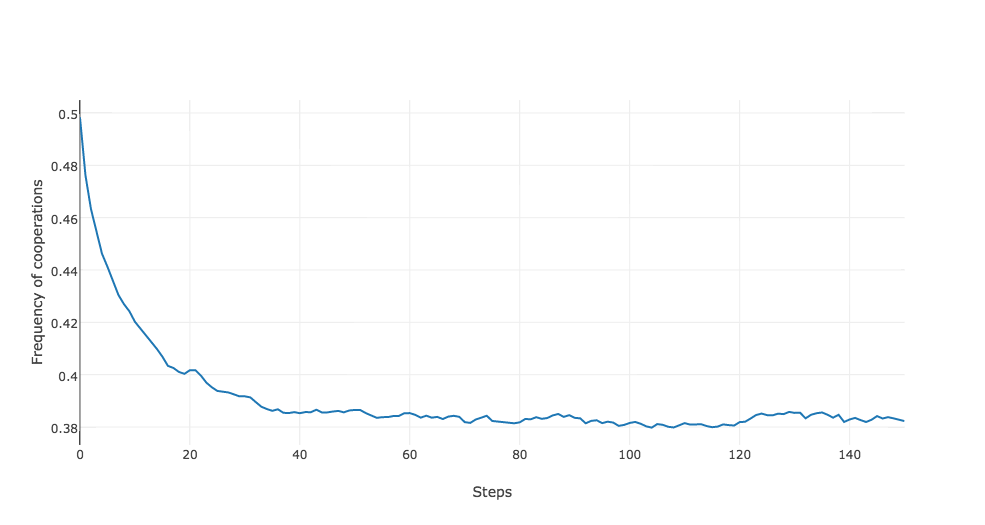
\includegraphics[width=\textwidth]{img/part2/part2-moore-notmyself.png}
\end{figure}

We can see that starting at $0.5$, slowly going to around a stationary state of $0.39$.

\subsubsection{Same in every run ?}

\begin{figure}[H]
\centering
   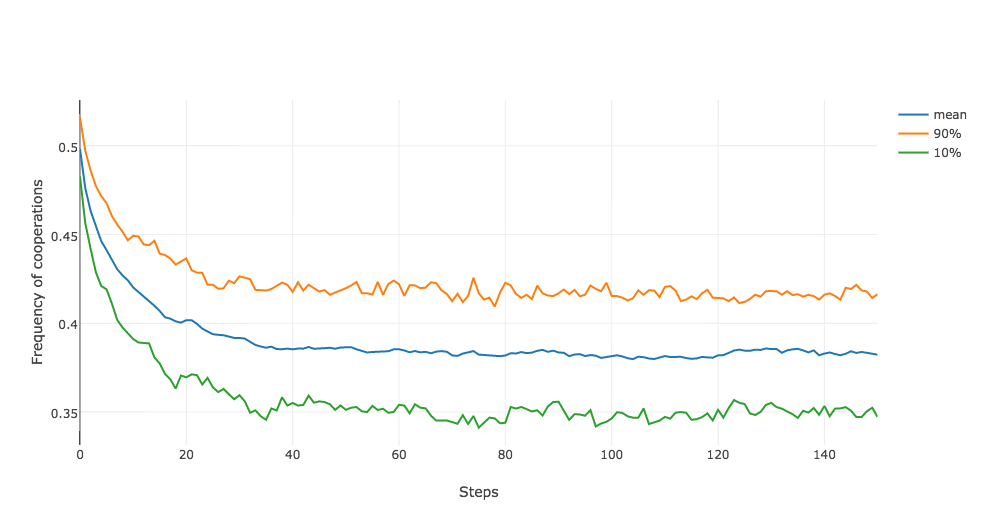
\includegraphics[width=\textwidth]{img/part2/part2-moore-notmyself-std.png}
\end{figure}

As above, answering the question \textit{is it approximately the same} is quite hard because it can be subjective. Above, it is plotted the $0.1$ and $0.9$ quantile. From this plot, one could reasonably say that it is in fact "approximately the same". Note that the $0.1$ and $0.9$ quantile has been chosen because the minimum would be at $0$ and the maximum at $1$.

\subsection{Visualization}

In the visualization below, red is cooperation and blue is defection. More visualization than asked has been plotted in order to see the stabilisation.

\subsubsection{t=0}

\begin{figure}[H]
\centering
   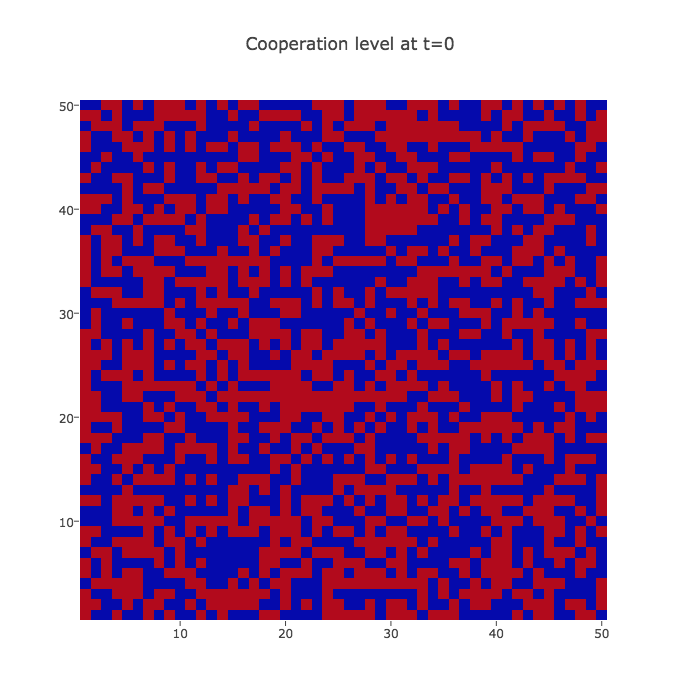
\includegraphics[width=0.6\textwidth]{img/part2/part2-moore-visu-0.png}
\end{figure}

\subsubsection{t=1}

\begin{figure}[H]
\centering
   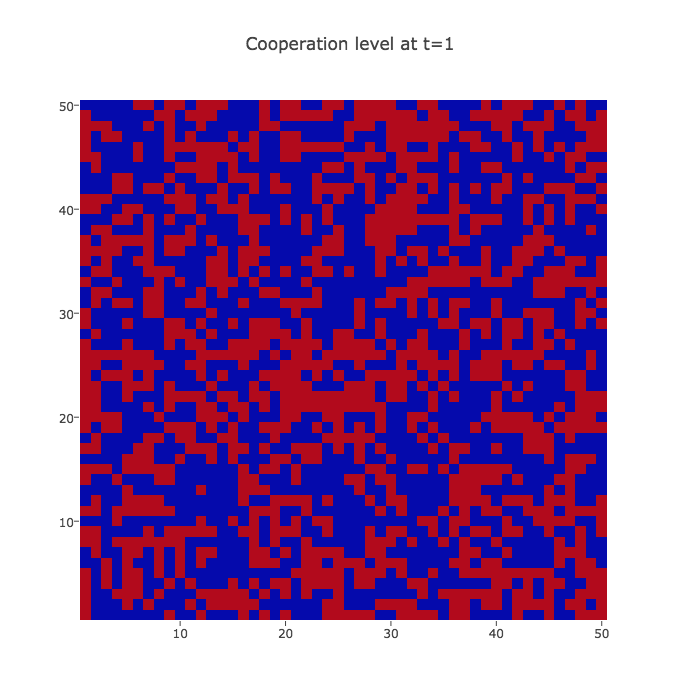
\includegraphics[width=0.6\textwidth]{img/part2/part2-moore-visu-1.png}
\end{figure}

\subsubsection{t=10}

\begin{figure}[H]
\centering
   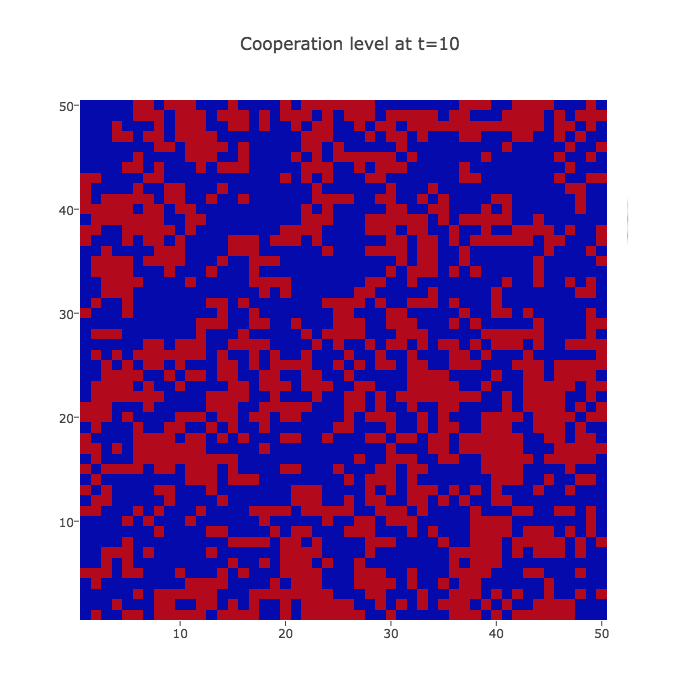
\includegraphics[width=0.6\textwidth]{img/part2/part2-moore-visu-10.png}
\end{figure}

\subsubsection{t=20}

\begin{figure}[H]
\centering
   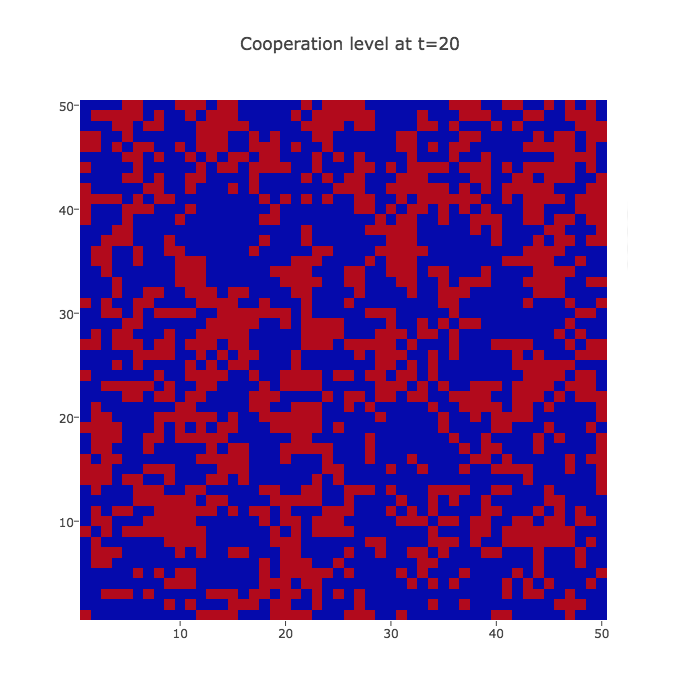
\includegraphics[width=0.6\textwidth]{img/part2/part2-moore-visu-20.png}
\end{figure}

\subsubsection{t=50}

\begin{figure}[H]
\centering
   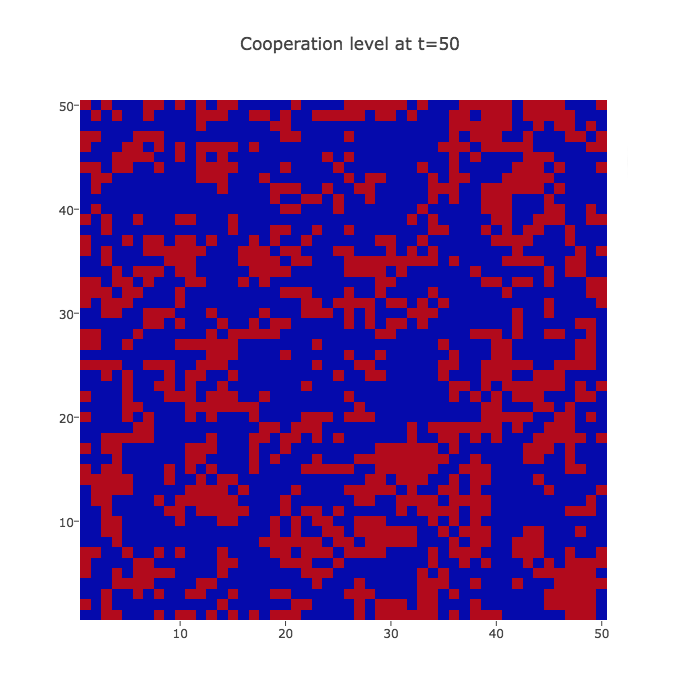
\includegraphics[width=0.6\textwidth]{img/part2/part2-moore-visu-50.png}
\end{figure}

\subsubsection{t=100}

\begin{figure}[H]
\centering
   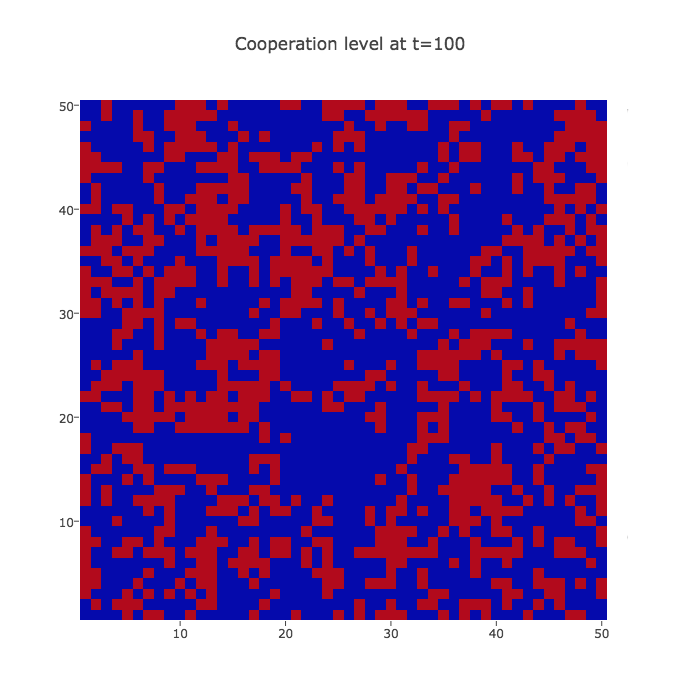
\includegraphics[width=0.6\textwidth]{img/part2/part2-moore-visu-100.png}
\end{figure}

\subsubsection{t=200}

\begin{figure}[H]
\centering
   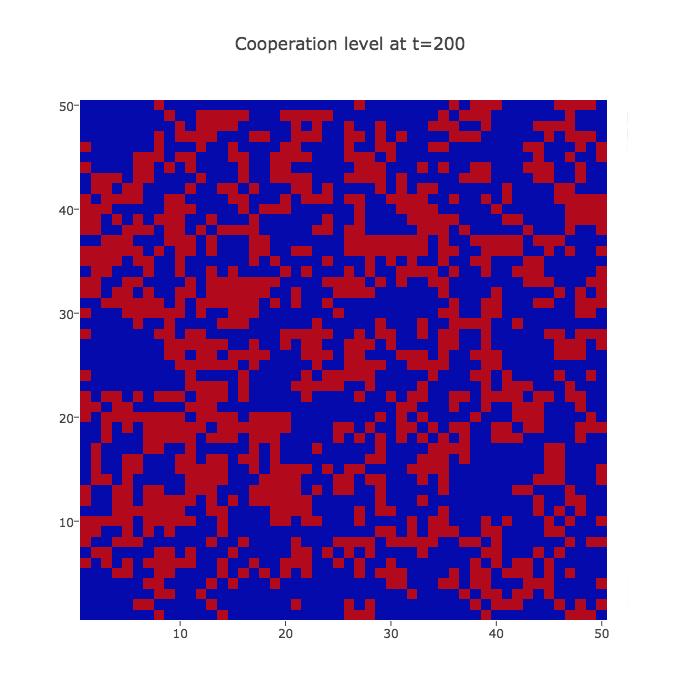
\includegraphics[width=0.6\textwidth]{img/part2/part2-moore-visu-200.png}
\end{figure}

\subsubsection{t=300}

\begin{figure}[H]
\centering
   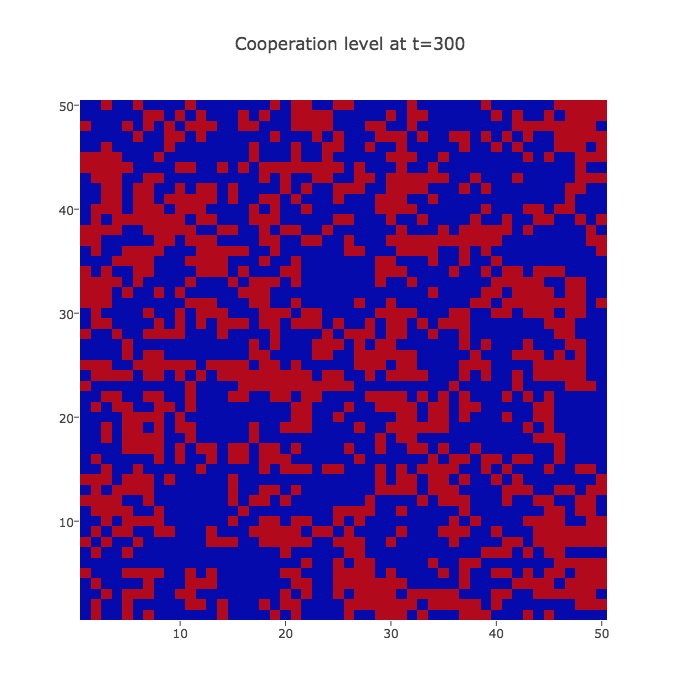
\includegraphics[width=0.6\textwidth]{img/part2/part2-moore-visu-300.png}
\end{figure}

\subsubsection{Comment}

For the visualisation on this part, we can see that no spatial structure like above are appearing like in part 1 of this assignment. The strategy here is more individual. According to the paper, it is due to small interaction neighborhood in the population (looking like filaments). It is because here it is advantageous to adopt a strategy that is opposite to the neighbour. In the paper, this is call a dendritic paper.

\subsection{Lattice size}

\subsubsection{4x4}

\begin{figure}[H]
   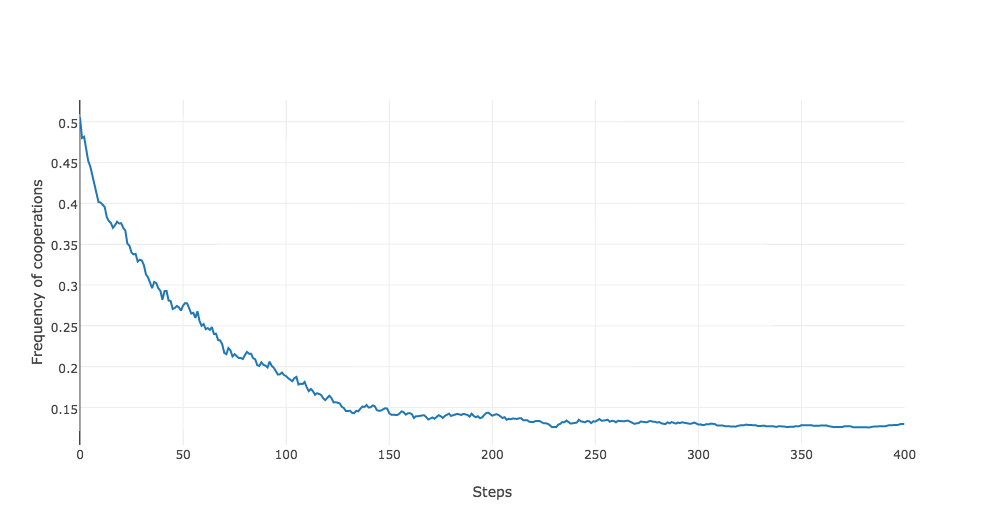
\includegraphics[width=0.7\textwidth]{img/part2/part2-moore-4-4.png}
\end{figure}
The stationary state seems to be near $0.08$. Here the lattice is very small, It could be wise to not put importance in this result.

\subsubsection{8x8}

\begin{figure}[H]
\centering
   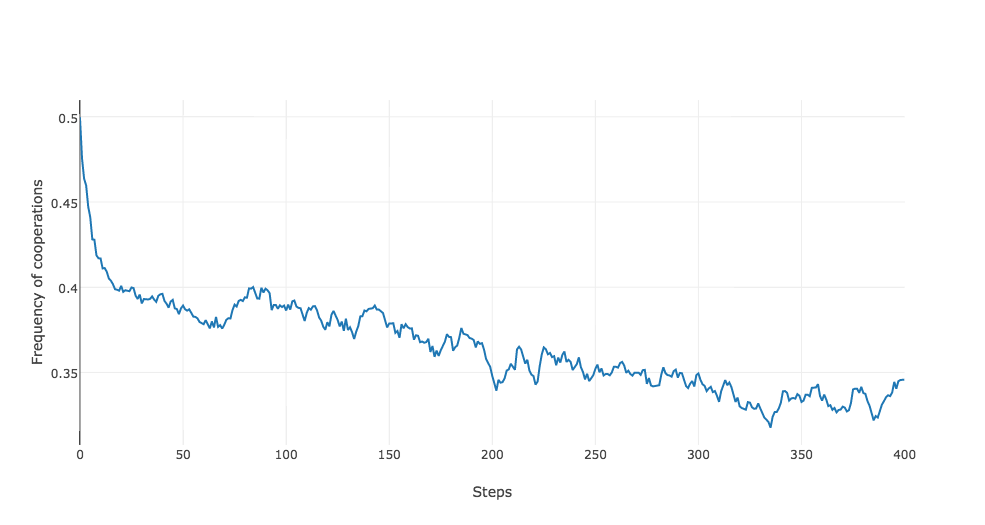
\includegraphics[width=0.7\textwidth]{img/part2/part2-moore-8-8.png}
\end{figure}
The stationary state seems to be near $0.32$. Here it is hard to find a stationary value seems there is a lot of little variation even for 100 iterations.


\subsubsection{12x12}

\begin{figure}[H]
\centering
   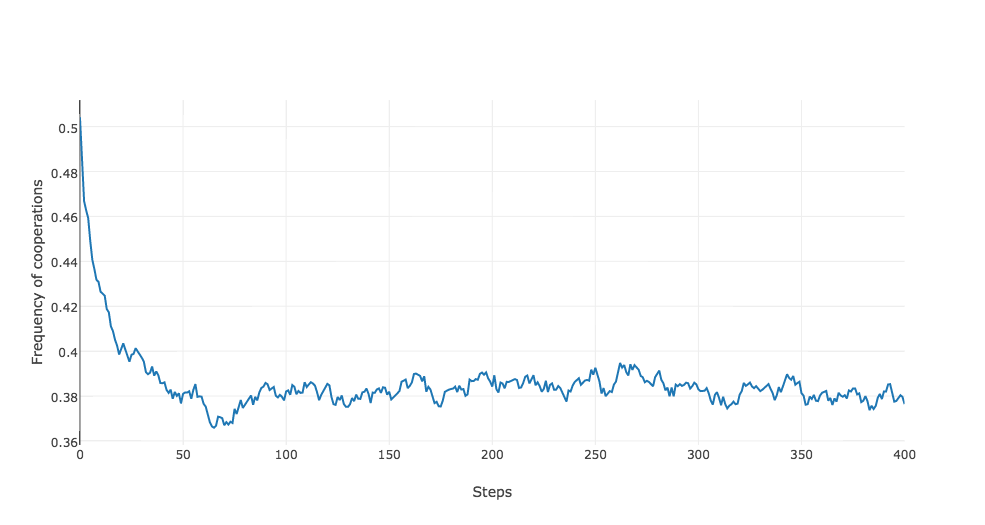
\includegraphics[width=0.7\textwidth]{img/part2/part2-moore-12-12.png}
\end{figure}
The stationary state seems to be near $0.38$. 

\subsubsection{20x20}

\begin{figure}[H]
\centering
   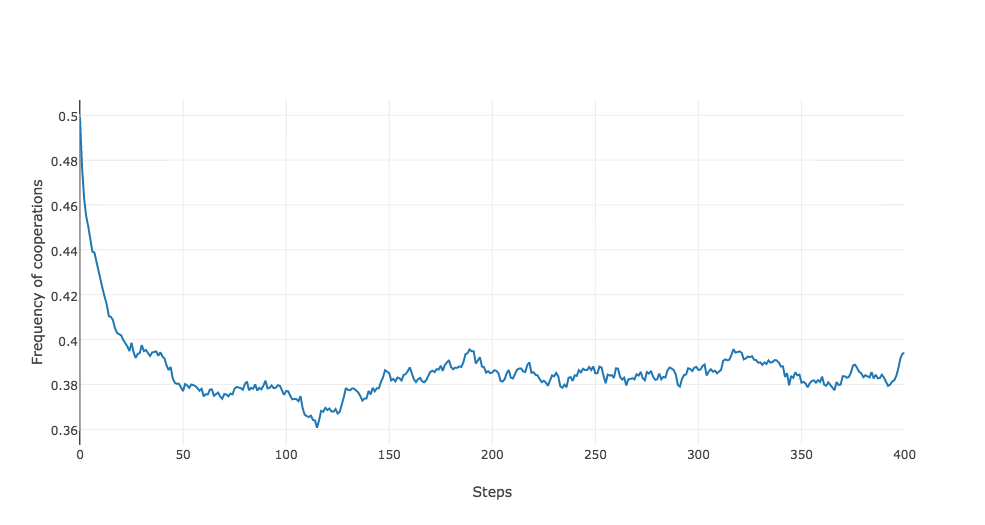
\includegraphics[width=0.7\textwidth]{img/part2/part2-moore-20-20.png}
\end{figure}

The stationary state seems to be near $0.38$. 

\subsubsection{Explanation}

Except for very small lattice, the level of cooperation seems to be the same. It matches the result above in the matrix visualisation where one could see the result to be individual.

\subsection{Von Neumann}

\begin{figure}[H]
\centering
   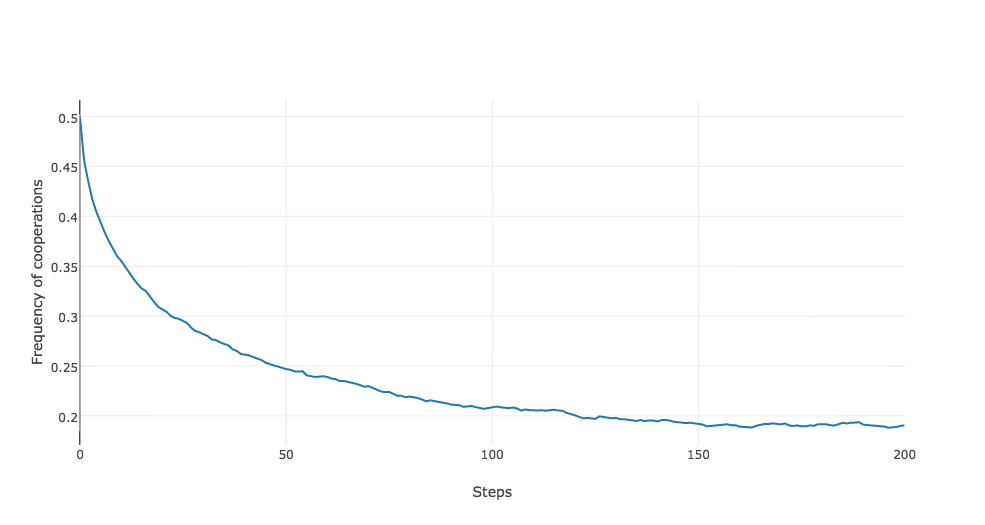
\includegraphics[width=0.8\textwidth]{img/part2/part2-vonn-notmyself.png}
\end{figure}

The level of cooperation seem to change with Van Neuman neighbourhood yielding approximately half of the value and converging in about the same time. According to the paper it is because cooperators tends to play an opposite strategy to its neighbor thus generating structure more advantageous to defector.

\section{Part 3 : Bonus}

For this project, it was asked of us to explore more parameters than those described in the exercise requirement.
I though that it would be relevant to explore if : 
\begin{itemize}
	\item The initial frequency of cooperation has an influence on the result.
	\item The lattice boundary has an influence on the result.
	\item The player playing with himself influence on the result.
\end{itemize}

\subsection{Initial frequency of cooperation}

Here we consider that the lattice has an initial frequency of cooperation of $Fc$ and we use the prisoner dilemma on a matrix of $50x50$.


\subsubsection{Initial Fc 0.9}

\begin{figure}[H]
\centering
   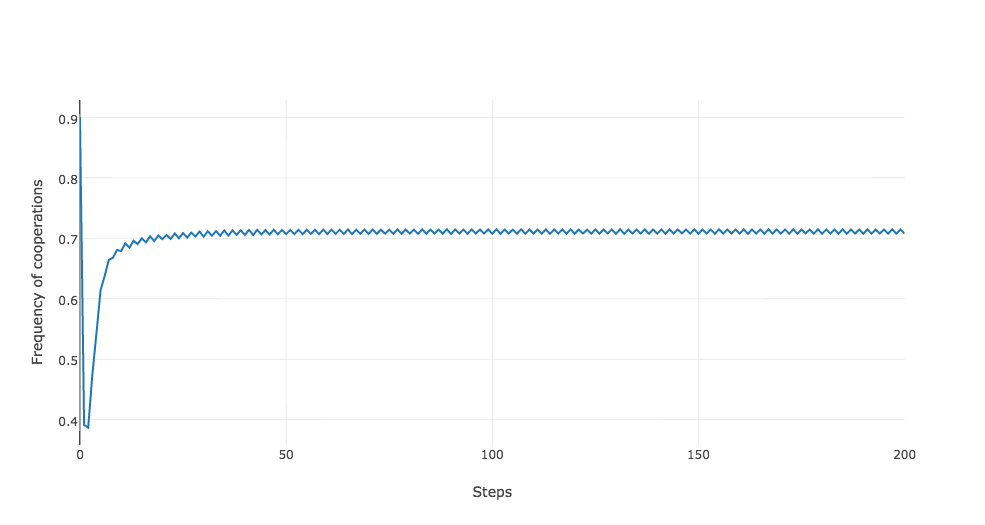
\includegraphics[width=0.8\textwidth]{img/part3/bonus-01-D.png}
\end{figure}

\subsubsection{Initial Fc 0.8}

\begin{figure}[H]
\centering
   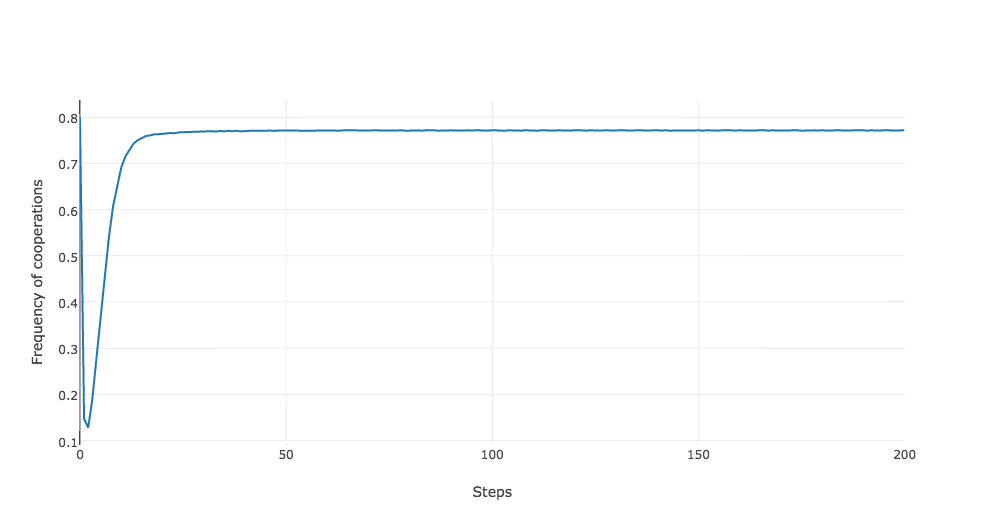
\includegraphics[width=0.8\textwidth]{img/part3/bonus-02-D.png}
\end{figure}

\subsubsection{Initial Fc 0.2}

\begin{figure}[H]
\centering
   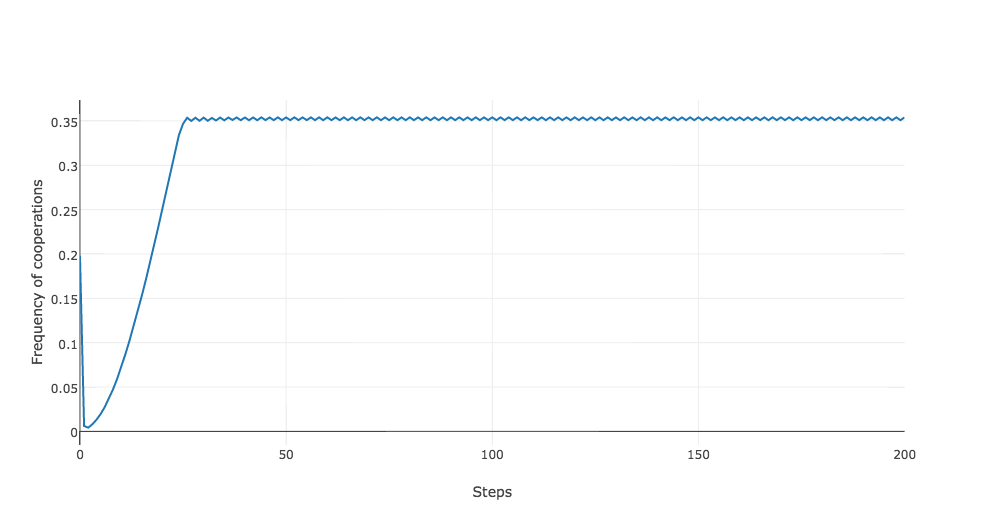
\includegraphics[width=0.8\textwidth]{img/part3/bonus-08-D.png}
\end{figure}

\subsubsection{Initial Fc 0.1}

\begin{figure}[H]
\centering
   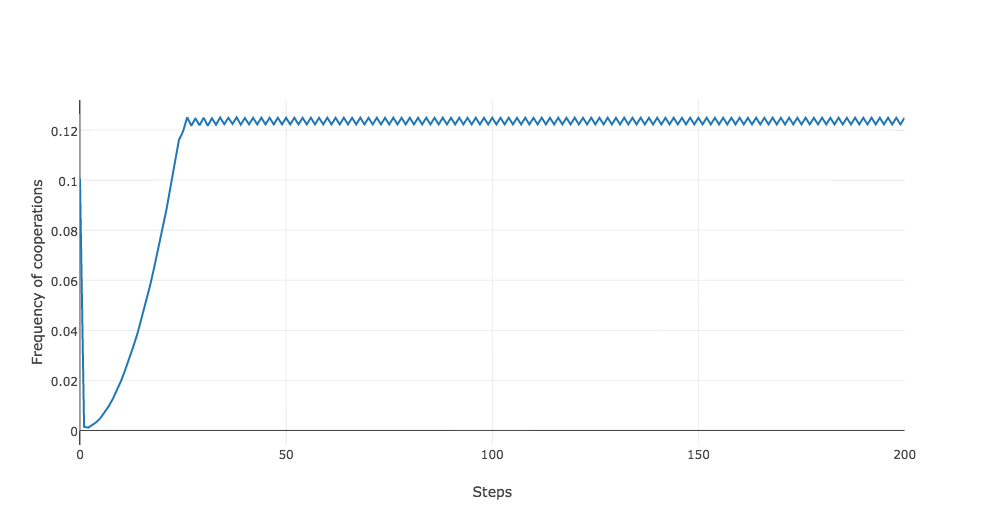
\includegraphics[width=0.8\textwidth]{img/part3/bonus-09-D.png}
\end{figure}

\subsubsection{Explanation}

Without surprise, the initial frequency of cooperation has an effect on the stationary frequency of cooperation. Indeed the less the matrix has cooperation, the lesser the chance of one player to cooperate with it's neighbour and the lesser the chance of formation of clusters as seen in part 1.


\subsection{Lattice boundary}

Here we consider that the lattice has boundary and we use the prisoner dilemma on a matrix of $50x50$ with a Moore neighborhood.

\subsubsection{Moore}

\begin{figure}[H]
\centering
   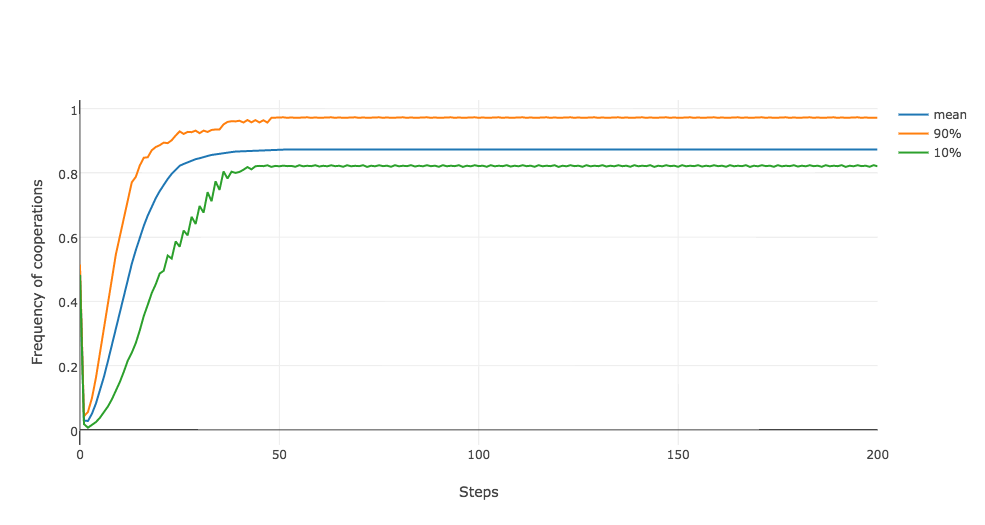
\includegraphics[width=0.8\textwidth]{img/part3/moore-bounded.png}
\end{figure}

\subsubsection{Von Neumann}

\begin{figure}[H]
\centering
   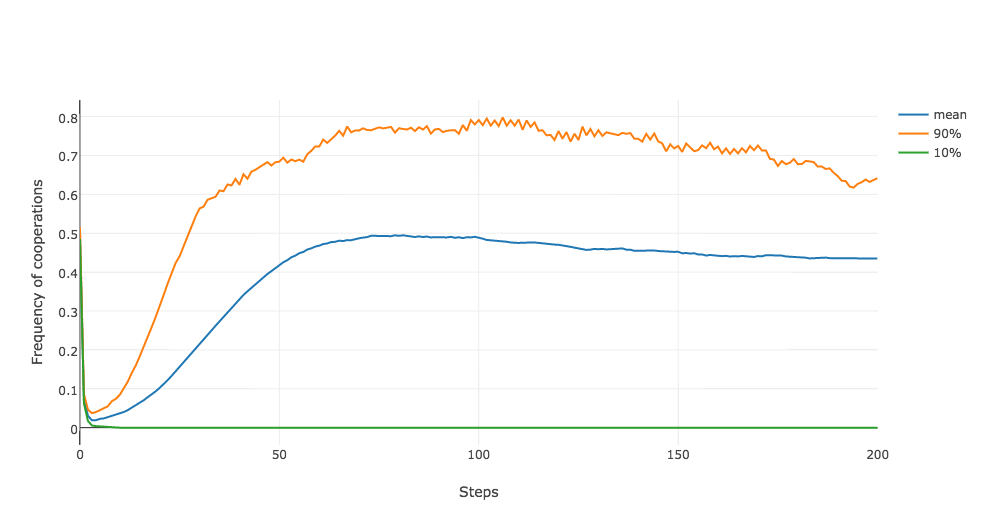
\includegraphics[width=0.8\textwidth]{img/part3/von-neuman-bouded.png}
\end{figure}

\subsubsection{Explanation}

The bound does not seem to have an influence or a negligible one on the stationary frequency of cooperation.

\subsection{Player playing with himself}

Here we consider that the player plays also with himself and we use the prisoner dilemma on a matrix of $50x50$ with a Van Neumann neighborhood.


\subsubsection{Von Neumann}

\begin{figure}[H]
\centering
   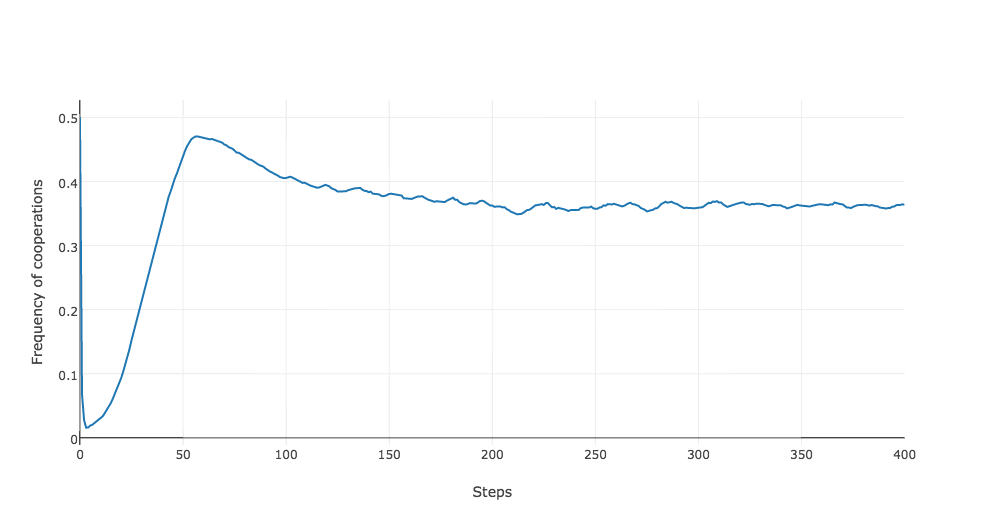
\includegraphics[width=0.8\textwidth]{img/part1/cf-vonn-myselfincluded.png}
\end{figure}

\subsubsection{Explanation}

With a little bit of counterintuition here, when the player plays with himself. One explanation could be that for example if a defector is around only cooperator : if he does not play with himself he will cooperate but if he plays with himself he will continue to defect.

\end{document}







































              